%=====================================================================
% Modelo de datos · Del diagrama entidad-relación al modelo
%=====================================================================
\subsection*{Del diagrama entidad-relación al modelo}
\addcontentsline{toc}{subsection}{Del diagrama entidad-relación al modelo}

El diagrama entidad-relación de partida, que se reproduce al final de esta subsección, tiene seis entidades —\textit{Usuario}, \textit{Skin}, \textit{Estadísticas}, \textit{Partida}, \textit{Reporte} y \textit{Baneo}— y nueve relaciones. Es anterior a los casos de uso, y varias decisiones de diseño lo cambiaron después (\mbox{D-02} a \mbox{D-06}). La tabla indica qué fue de cada elemento del diagrama; el diagrama actualizado está en la subsección siguiente. Todo lo que el diagrama no tenía —sesiones, tokens, bitácoras, relaciones entre jugadores, salas, economía y tutorial— lo exigen los casos de uso, y la Matriz 1 de trazabilidad indica cuál.

\begin{center}\small
\begin{longtable}{|L{0.21\textwidth}|L{0.30\textwidth}|L{0.39\textwidth}|}
\hline
\textbf{Elemento del diagrama} & \textbf{En el modelo} & \textbf{Qué cambió y por qué} \\ \hline
\endfirsthead
\hline
\textbf{Elemento del diagrama} & \textbf{En el modelo} & \textbf{Qué cambió y por qué} \\ \hline
\endhead
\textit{Usuario} & \textit{Usuario} & Se elimina el atributo compuesto \at{nombre\_completo} y, con él, \at{nombre}, \at{apellido\_paterno} y \at{apellido\_materno}, junto con \at{region}: ningún flujo los usa (\mbox{D-06}). Se elimina \at{edad}, que es derivada. \at{contraseña} pasa a \at{contrasena\_hash} y \at{contrasena\_sal}. Se añaden \at{tipo\_cuenta} para el invitado (\mbox{D-02}), \at{rol}, y los datos del bloqueo, la verificación y la progresión. \\ \hline
\textit{Skin} & \textit{Ranura}, \textit{ObjetoCosmetico} & Un solo tipo de skin no alcanza para seis ranuras de personalización (\mbox{D-03}). El atributo \at{tipo} del skin se convierte en la entidad \textit{Ranura}; \at{costo} pasa a \at{precio}. \\ \hline
Posee (N:M) & \textit{UsuarioObjeto} & Se conserva como entidad asociativa con su \at{fecha\_obtencion} y gana \at{origen}. \\ \hline
Equipa (N:1) & \textit{Equipamiento} & Un skin equipado por usuario pasa a ser un objeto equipado por cada ranura: una fila por usuario y ranura. \\ \hline
\textit{Estadísticas}, Tiene (1:1) & \textit{Modo}, \textit{EstadisticaModo} & El elo y los contadores son por modo (\mbox{D-04}), así que la relación deja de ser 1:1: hay una fila por usuario y modo. Se elimina \at{porcentaje\_victorias}, que es derivado. \\ \hline
\textit{Partida} & \textit{Partida} & \at{num\_jugadores} pasa a \textit{Modo}, del que depende. \at{duracion} se elimina porque se calcula. Se añaden \at{tipo}, \at{forma\_termino}, el reloj y los datos de las partidas contra la IA (\mbox{D-12}). \\ \hline
Participa (N:M, 2 a 4) & \textit{Participacion} & \at{color\_ficha} pasa a \at{simbolo\_peon} y \at{barreras\_restantes} a \at{muros\_restantes}. Se añaden el elo de entrada y de salida, el reloj y el estado de conexión. La cardinalidad baja a 1 a 4, porque en una partida contra la IA solo participa el jugador. \\ \hline
\textit{Reporte}, Emite (1:N), Señala (N:1), Sobre (N:1) & \textit{Reporte}, \textit{MotivoReporte} & Las tres relaciones quedan como las llaves foráneas \at{id\_denunciante}, \at{id\_reportado} e \at{id\_partida}; la partida adjunta tiene que ser una que jugaron los dos (\mbox{CU-42} \mbox{RN-09}). El \at{motivo} en texto pasa a un catálogo; \at{estado\_reporte} pasa a \at{estado} con el moderador que lo revisa. \\ \hline
\textit{Baneo}, Recibe (1:N), Origina (N:1) & \textit{Sancion}, \textit{Apelacion} & La sanción gana ámbito de cuenta o de chat (\mbox{D-05}). \at{num\_reportes} y \at{activo} se eliminan: el primero es un conteo y el segundo se deducía de las fechas. La relación Origina queda como \at{id\_reporte}. \\ \hline
\end{longtable}
\end{center}

\begin{landscape}
\subsubsection*{Diagrama original}
\addcontentsline{toc}{subsubsection}{Diagrama original}
El diagrama entidad-relación de partida, en notación de Chen, dibujado de nuevo a partir de su modelo (\at{er/\allowbreak{}modelos/\allowbreak{}original.py}) con los mismos renderizadores que los diagramas actualizados.
\begin{center}
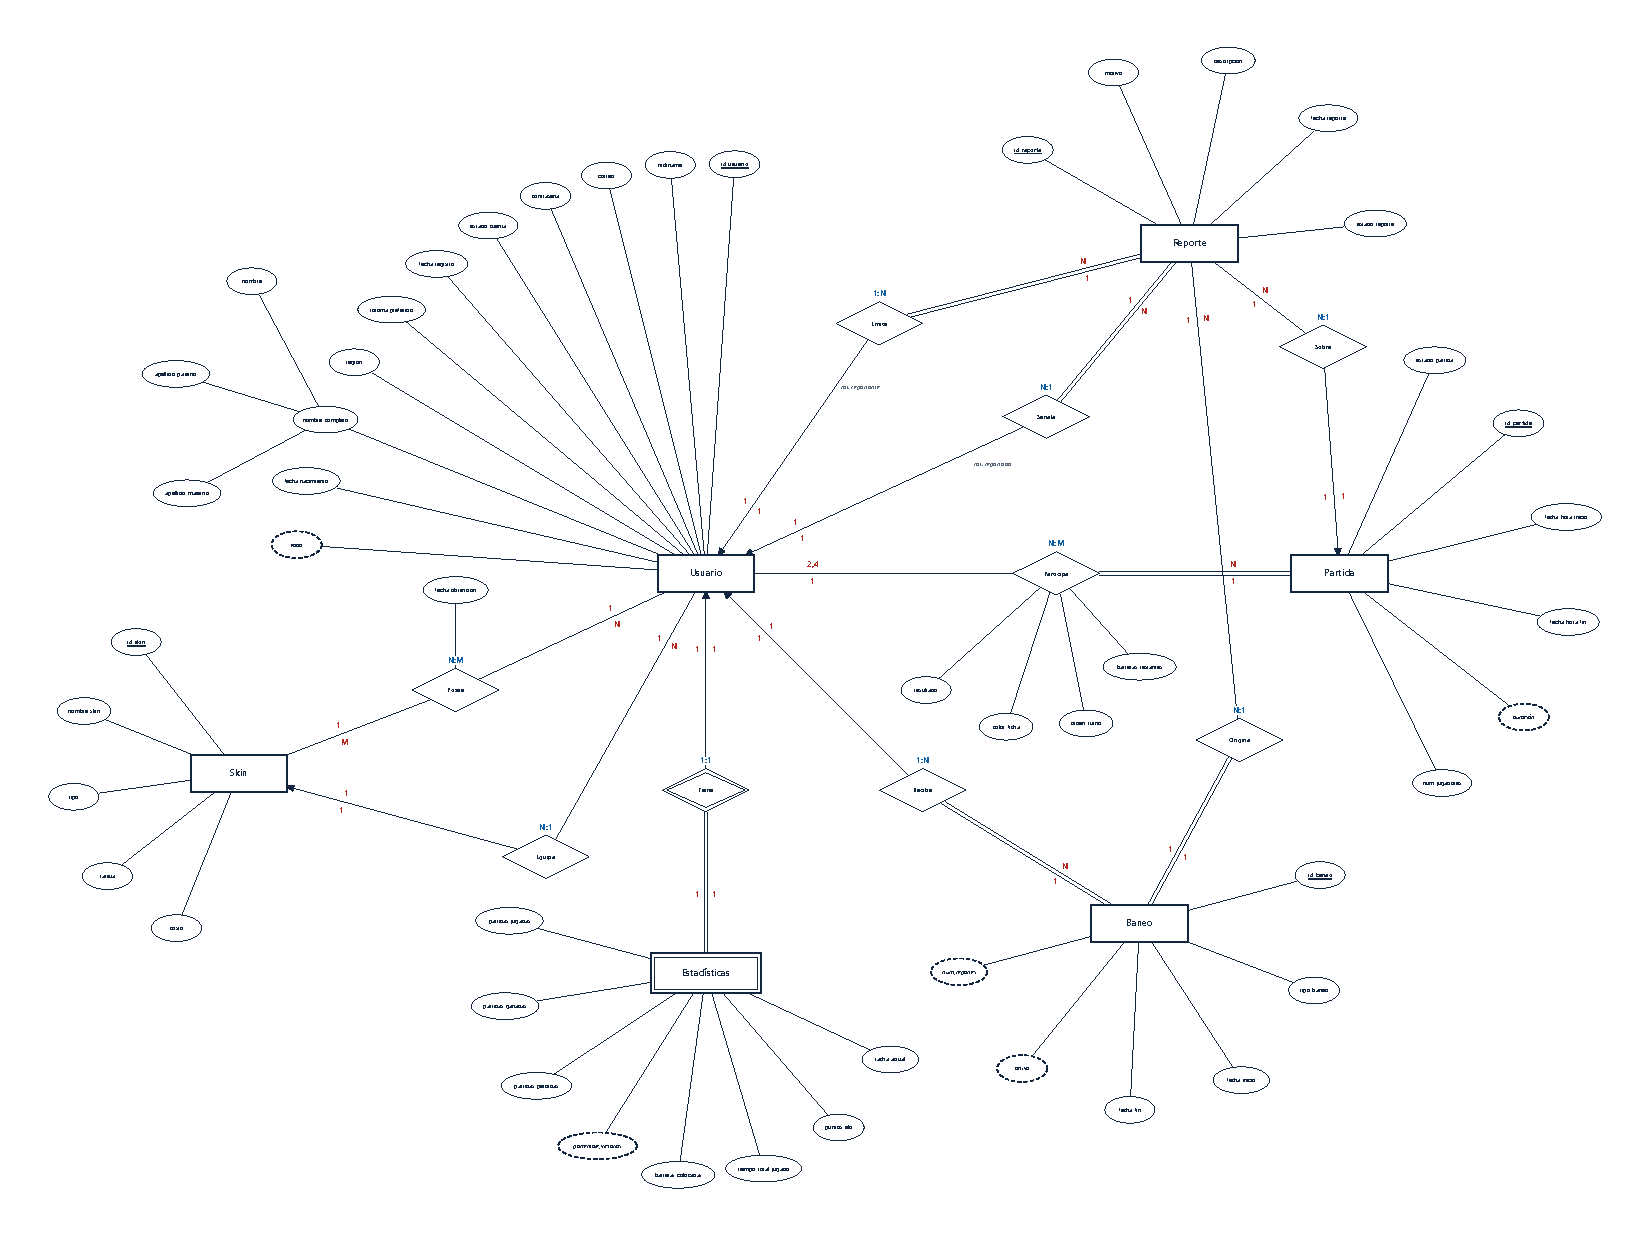
\includegraphics[width=\linewidth,height=0.8\textheight,keepaspectratio]{er/salida/original}
\end{center}
\end{landscape}
